\documentclass[10pt]{standalone}
\usepackage{commands}

\begin{document}
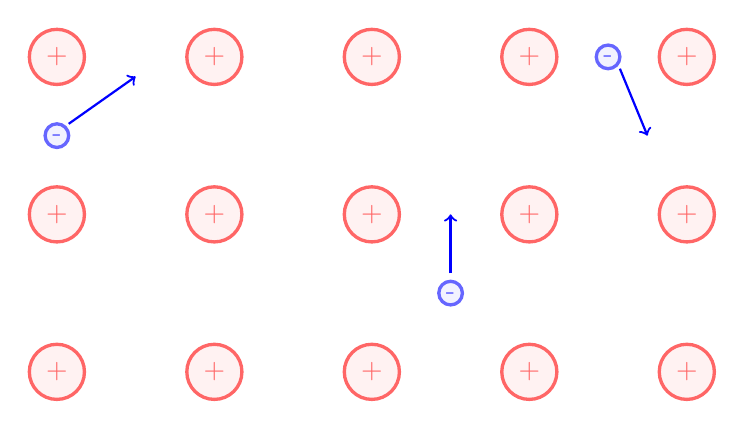
\begin{tikzpicture}[scale=1]
    \draw[color=red!60, fill=red!5, very thick] (-4, 0) circle (.35cm) node {+};
    \draw[color=red!60, fill=red!5, very thick] (-2, 0) circle (.35cm) node {+};
    \draw[color=red!60, fill=red!5, very thick] (0, 0) circle (.35cm) node {+};
    \draw[color=red!60, fill=red!5, very thick] (2, 0) circle (.35cm) node {+};
    \draw[color=red!60, fill=red!5, very thick] (4, 0) circle (.35cm) node {+};
    \draw[color=red!60, fill=red!5, very thick] (-4, 2) circle (.35cm) node {+};
    \draw[color=red!60, fill=red!5, very thick] (-2, 2) circle (.35cm) node {+};
    \draw[color=red!60, fill=red!5, very thick] (0, 2) circle (.35cm) node {+};
    \draw[color=red!60, fill=red!5, very thick] (2, 2) circle (.35cm) node {+};
    \draw[color=red!60, fill=red!5, very thick] (4, 2) circle (.35cm) node {+};
    \draw[color=red!60, fill=red!5, very thick] (-4, -2) circle (.35cm) node {+};
    \draw[color=red!60, fill=red!5, very thick] (-2, -2) circle (.35cm) node {+};
    \draw[color=red!60, fill=red!5, very thick] (0, -2) circle (.35cm) node {+};
    \draw[color=red!60, fill=red!5, very thick] (2, -2) circle (.35cm) node {+};
    \draw[color=red!60, fill=red!5, very thick] (4, -2) circle (.35cm) node {+};
    \draw[color=blue!60, fill=blue!5, very thick] (1,-1) circle (.15cm) node {-};
    \draw[blue, ->, thick] (1, -0.75) -- (1, 0);
    \draw[color=blue!60, fill=blue!5, very thick] (-4,1) circle (.15cm) node {-};
    \draw[blue, ->, thick] (-3.85, 1.15) -- (-3, 1.75);
    \draw[color=blue!60, fill=blue!5, very thick] (3,2) circle (.15cm) node {-};
    \draw[blue, ->, thick] (3.15, 1.85) -- (3.5, 1);
\end{tikzpicture}
\end{document}